\documentclass[]{article}
\usepackage{lmodern}
\usepackage{amssymb,amsmath}
\usepackage{ifxetex,ifluatex}
\usepackage{fixltx2e} % provides \textsubscript
\ifnum 0\ifxetex 1\fi\ifluatex 1\fi=0 % if pdftex
  \usepackage[T1]{fontenc}
  \usepackage[utf8]{inputenc}
\else % if luatex or xelatex
  \ifxetex
    \usepackage{mathspec}
  \else
    \usepackage{fontspec}
  \fi
  \defaultfontfeatures{Ligatures=TeX,Scale=MatchLowercase}
\fi
% use upquote if available, for straight quotes in verbatim environments
\IfFileExists{upquote.sty}{\usepackage{upquote}}{}
% use microtype if available
\IfFileExists{microtype.sty}{%
\usepackage{microtype}
\UseMicrotypeSet[protrusion]{basicmath} % disable protrusion for tt fonts
}{}
\usepackage[margin=1in]{geometry}
\usepackage{hyperref}
\hypersetup{unicode=true,
            pdftitle={Lab 4},
            pdfauthor={Eric Yuan, qy2205},
            pdfborder={0 0 0},
            breaklinks=true}
\urlstyle{same}  % don't use monospace font for urls
\usepackage{color}
\usepackage{fancyvrb}
\newcommand{\VerbBar}{|}
\newcommand{\VERB}{\Verb[commandchars=\\\{\}]}
\DefineVerbatimEnvironment{Highlighting}{Verbatim}{commandchars=\\\{\}}
% Add ',fontsize=\small' for more characters per line
\usepackage{framed}
\definecolor{shadecolor}{RGB}{248,248,248}
\newenvironment{Shaded}{\begin{snugshade}}{\end{snugshade}}
\newcommand{\AlertTok}[1]{\textcolor[rgb]{0.94,0.16,0.16}{#1}}
\newcommand{\AnnotationTok}[1]{\textcolor[rgb]{0.56,0.35,0.01}{\textbf{\textit{#1}}}}
\newcommand{\AttributeTok}[1]{\textcolor[rgb]{0.77,0.63,0.00}{#1}}
\newcommand{\BaseNTok}[1]{\textcolor[rgb]{0.00,0.00,0.81}{#1}}
\newcommand{\BuiltInTok}[1]{#1}
\newcommand{\CharTok}[1]{\textcolor[rgb]{0.31,0.60,0.02}{#1}}
\newcommand{\CommentTok}[1]{\textcolor[rgb]{0.56,0.35,0.01}{\textit{#1}}}
\newcommand{\CommentVarTok}[1]{\textcolor[rgb]{0.56,0.35,0.01}{\textbf{\textit{#1}}}}
\newcommand{\ConstantTok}[1]{\textcolor[rgb]{0.00,0.00,0.00}{#1}}
\newcommand{\ControlFlowTok}[1]{\textcolor[rgb]{0.13,0.29,0.53}{\textbf{#1}}}
\newcommand{\DataTypeTok}[1]{\textcolor[rgb]{0.13,0.29,0.53}{#1}}
\newcommand{\DecValTok}[1]{\textcolor[rgb]{0.00,0.00,0.81}{#1}}
\newcommand{\DocumentationTok}[1]{\textcolor[rgb]{0.56,0.35,0.01}{\textbf{\textit{#1}}}}
\newcommand{\ErrorTok}[1]{\textcolor[rgb]{0.64,0.00,0.00}{\textbf{#1}}}
\newcommand{\ExtensionTok}[1]{#1}
\newcommand{\FloatTok}[1]{\textcolor[rgb]{0.00,0.00,0.81}{#1}}
\newcommand{\FunctionTok}[1]{\textcolor[rgb]{0.00,0.00,0.00}{#1}}
\newcommand{\ImportTok}[1]{#1}
\newcommand{\InformationTok}[1]{\textcolor[rgb]{0.56,0.35,0.01}{\textbf{\textit{#1}}}}
\newcommand{\KeywordTok}[1]{\textcolor[rgb]{0.13,0.29,0.53}{\textbf{#1}}}
\newcommand{\NormalTok}[1]{#1}
\newcommand{\OperatorTok}[1]{\textcolor[rgb]{0.81,0.36,0.00}{\textbf{#1}}}
\newcommand{\OtherTok}[1]{\textcolor[rgb]{0.56,0.35,0.01}{#1}}
\newcommand{\PreprocessorTok}[1]{\textcolor[rgb]{0.56,0.35,0.01}{\textit{#1}}}
\newcommand{\RegionMarkerTok}[1]{#1}
\newcommand{\SpecialCharTok}[1]{\textcolor[rgb]{0.00,0.00,0.00}{#1}}
\newcommand{\SpecialStringTok}[1]{\textcolor[rgb]{0.31,0.60,0.02}{#1}}
\newcommand{\StringTok}[1]{\textcolor[rgb]{0.31,0.60,0.02}{#1}}
\newcommand{\VariableTok}[1]{\textcolor[rgb]{0.00,0.00,0.00}{#1}}
\newcommand{\VerbatimStringTok}[1]{\textcolor[rgb]{0.31,0.60,0.02}{#1}}
\newcommand{\WarningTok}[1]{\textcolor[rgb]{0.56,0.35,0.01}{\textbf{\textit{#1}}}}
\usepackage{graphicx,grffile}
\makeatletter
\def\maxwidth{\ifdim\Gin@nat@width>\linewidth\linewidth\else\Gin@nat@width\fi}
\def\maxheight{\ifdim\Gin@nat@height>\textheight\textheight\else\Gin@nat@height\fi}
\makeatother
% Scale images if necessary, so that they will not overflow the page
% margins by default, and it is still possible to overwrite the defaults
% using explicit options in \includegraphics[width, height, ...]{}
\setkeys{Gin}{width=\maxwidth,height=\maxheight,keepaspectratio}
\IfFileExists{parskip.sty}{%
\usepackage{parskip}
}{% else
\setlength{\parindent}{0pt}
\setlength{\parskip}{6pt plus 2pt minus 1pt}
}
\setlength{\emergencystretch}{3em}  % prevent overfull lines
\providecommand{\tightlist}{%
  \setlength{\itemsep}{0pt}\setlength{\parskip}{0pt}}
\setcounter{secnumdepth}{0}
% Redefines (sub)paragraphs to behave more like sections
\ifx\paragraph\undefined\else
\let\oldparagraph\paragraph
\renewcommand{\paragraph}[1]{\oldparagraph{#1}\mbox{}}
\fi
\ifx\subparagraph\undefined\else
\let\oldsubparagraph\subparagraph
\renewcommand{\subparagraph}[1]{\oldsubparagraph{#1}\mbox{}}
\fi

%%% Use protect on footnotes to avoid problems with footnotes in titles
\let\rmarkdownfootnote\footnote%
\def\footnote{\protect\rmarkdownfootnote}

%%% Change title format to be more compact
\usepackage{titling}

% Create subtitle command for use in maketitle
\newcommand{\subtitle}[1]{
  \posttitle{
    \begin{center}\large#1\end{center}
    }
}

\setlength{\droptitle}{-2em}

  \title{Lab 4}
    \pretitle{\vspace{\droptitle}\centering\huge}
  \posttitle{\par}
    \author{Eric Yuan, qy2205}
    \preauthor{\centering\large\emph}
  \postauthor{\par}
      \predate{\centering\large\emph}
  \postdate{\par}
    \date{October 23, 2018}


\begin{document}
\maketitle

\hypertarget{instructions}{%
\section{Instructions}\label{instructions}}

Make sure that you upload a knitted pdf or html file to the canvas page
(this should have a .pdf or .html extension). Also upload the .Rmd file.
Include output for each question in its own individual code chunk and
don't print out any vector that has more than 20 elements.

Objectives: KNN Classification and Cross-Validation

\hypertarget{background}{%
\section{Background}\label{background}}

Today we'll be using the \emph{Weekly} dataset from the \emph{ISLR}
package. This data is similar to the \emph{Smarket} data from class. The
dataset contains \(1089\) weekly returns from the beginning of 1990 to
the end of 2010. Make sure that you have the \emph{ISLR} package
installed and loaded by running (without the code commented out) the
following:

\begin{Shaded}
\begin{Highlighting}[]
\CommentTok{# install.packages("ISLR")}
\KeywordTok{library}\NormalTok{(ISLR)}
\end{Highlighting}
\end{Shaded}

We'd like to see if we can accurately predict the direction of a week's
return based on the returns over the last five weeks. \emph{Today} gives
the percentage return for the week considered and \emph{Year} provides
the year that the observation was recorded. \emph{Lag1} - \emph{Lag5}
give the percentage return for 1 - 5 weeks previous and \emph{Direction}
is a factor variable indicating the direction (`UP' or `DOWN') of the
return for the week considered.

\hypertarget{part-1-visualizing-the-relationship-between-this-weeks-returns-and-the-previous-weeks-returns.}{%
\section{Part 1: Visualizing the relationship between this week's
returns and the previous week's
returns.}\label{part-1-visualizing-the-relationship-between-this-weeks-returns-and-the-previous-weeks-returns.}}

\begin{enumerate}
\def\labelenumi{\arabic{enumi}.}
\tightlist
\item
  Explore the relationship between a week's return and the previous
  week's return. You should plot more graphs for yourself, but include
  in the lab write-up a scatterplot of the returns for the weeks
  considered (\emph{Today}) vs the return from two weeks previous
  (\emph{Lag2}), and side-by-side boxplots for the lag one week previous
  (\emph{Lag1}) divided by the direction of this week's Reuther
  (\emph{Direction}).
\end{enumerate}

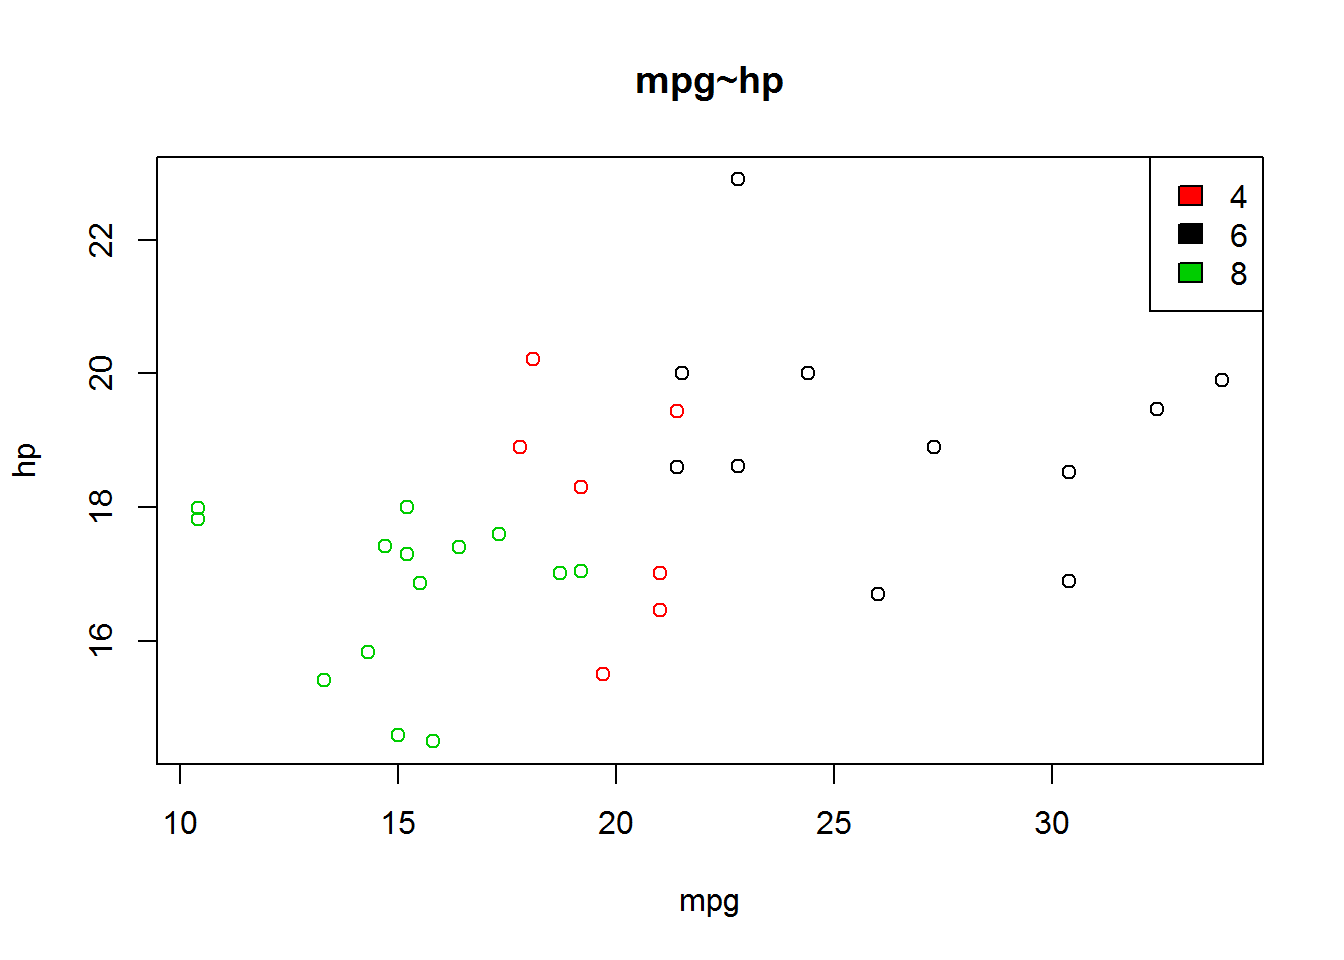
\includegraphics{Lab4_UNI_files/figure-latex/unnamed-chunk-3-1.pdf}
\includegraphics{Lab4_UNI_files/figure-latex/unnamed-chunk-3-2.pdf}

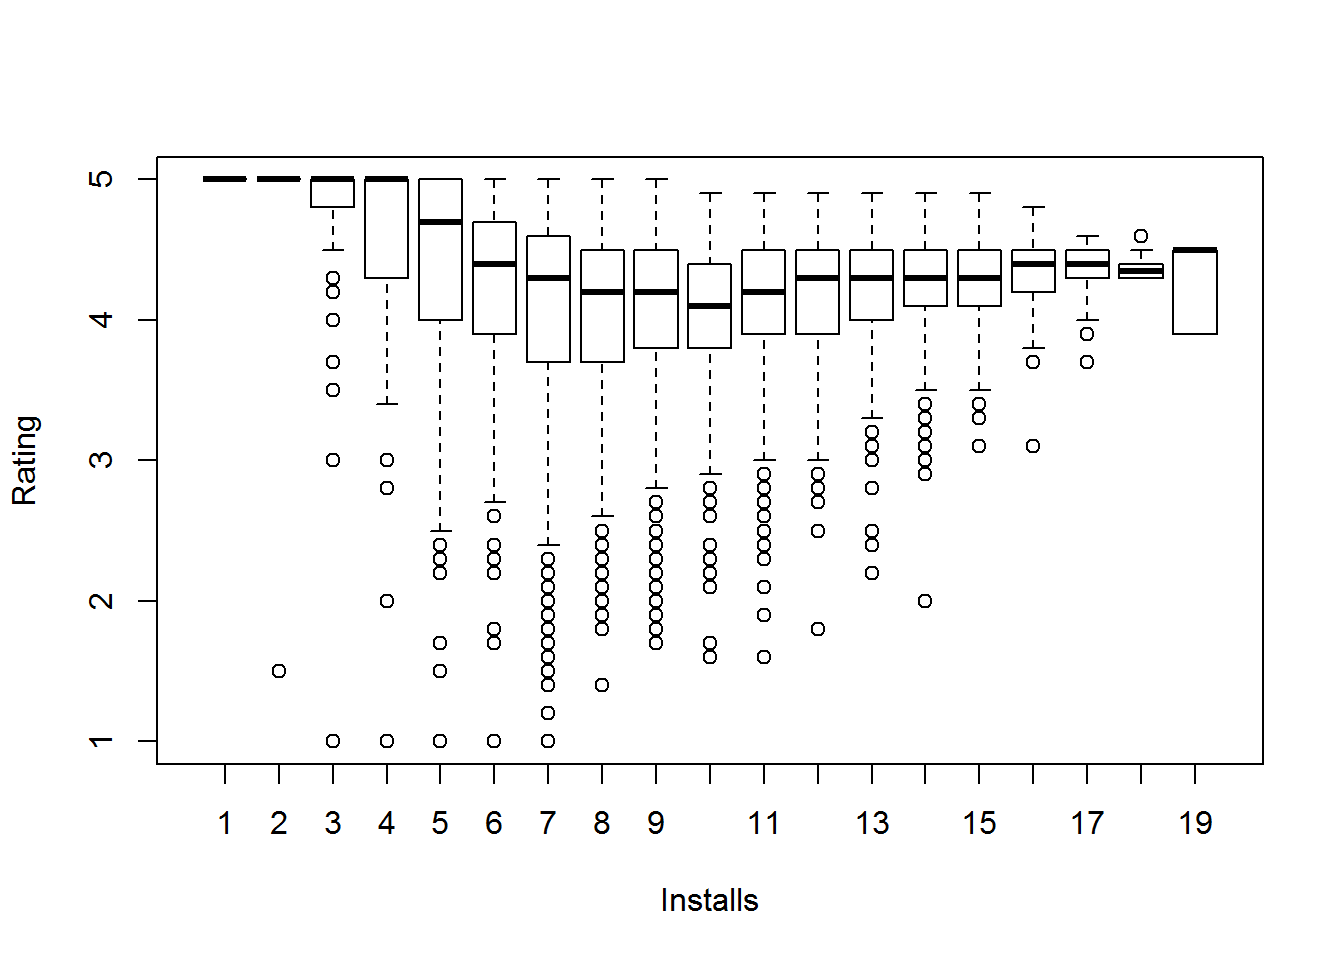
\includegraphics{Lab4_UNI_files/figure-latex/unnamed-chunk-4-1.pdf}
\includegraphics{Lab4_UNI_files/figure-latex/unnamed-chunk-4-2.pdf}

\hypertarget{part-2-building-a-classifier}{%
\section{Part 2: Building a
classifier}\label{part-2-building-a-classifier}}

Recall the KNN procedure. We classify a new point with the following
steps:

-- Calculate the Euclidean distance between the new point and all other
points.

-- Create the set \(\mathcal{N}_{new}\) containing the \(K\) closest
points (or, nearest neighbors) to the new point.

-- Determine the number of `UPs' and `DOWNs' in \(\mathcal{N}_{new}\)
and classify the new point according to the most frequent.

\begin{enumerate}
\def\labelenumi{\arabic{enumi}.}
\setcounter{enumi}{1}
\tightlist
\item
  We'd like to perform KNN on the \emph{Weekly} data, as we did with the
  \emph{Smarket} data in class. In class we wrote the following function
  which takes as input a new point \((Lag1_{new}, Lag2_{new})\) and
  provides the KNN decision using as defaults \(K=5\), Lag1 data given
  in \emph{Smarket\$Lag1}, and Lag2 data given in \emph{Smarket\$Lag2}.
  Update the function to calculate the KNN decision for weekly market
  direction using the \emph{Weekly} dataset with \emph{Lag1} -
  \emph{Lag5} as predictors. Your function should have only three input
  values: (1) a new point which should be a vector of length \(5\), (2)
  a value for K, and (3) the Lag data which should be a data frame with
  five columns (and n rows).
\end{enumerate}

\begin{Shaded}
\begin{Highlighting}[]
\NormalTok{ KNN.decision <-}\StringTok{ }\ControlFlowTok{function}\NormalTok{(Lag1.new, Lag2.new, }\DataTypeTok{K =} \DecValTok{5}\NormalTok{, }\DataTypeTok{Lag1 =}\NormalTok{ Smarket}\OperatorTok{$}\NormalTok{Lag1, }\DataTypeTok{Lag2 =}\NormalTok{ Smarket}\OperatorTok{$}\NormalTok{Lag2) \{}
   
\NormalTok{   n <-}\StringTok{ }\KeywordTok{length}\NormalTok{(Lag1)}
   
   \KeywordTok{stopifnot}\NormalTok{(}\KeywordTok{length}\NormalTok{(Lag2) }\OperatorTok{==}\StringTok{ }\NormalTok{n, }\KeywordTok{length}\NormalTok{(Lag1.new) }\OperatorTok{==}\StringTok{ }\DecValTok{1}\NormalTok{, }\KeywordTok{length}\NormalTok{(Lag2.new) }\OperatorTok{==}\StringTok{ }\DecValTok{1}\NormalTok{, K }\OperatorTok{<=}\StringTok{ }\NormalTok{n)}
   
\NormalTok{   dists       <-}\StringTok{ }\KeywordTok{sqrt}\NormalTok{((Lag1}\OperatorTok{-}\NormalTok{Lag1.new)}\OperatorTok{^}\DecValTok{2} \OperatorTok{+}\StringTok{ }\NormalTok{(Lag2}\OperatorTok{-}\NormalTok{Lag2.new)}\OperatorTok{^}\DecValTok{2}\NormalTok{)}
\NormalTok{   neighbors  <-}\StringTok{ }\KeywordTok{order}\NormalTok{(dists)[}\DecValTok{1}\OperatorTok{:}\NormalTok{K]}
\NormalTok{   neighb.dir <-}\StringTok{ }\NormalTok{Smarket}\OperatorTok{$}\NormalTok{Direction[neighbors]}
\NormalTok{   choice      <-}\StringTok{ }\KeywordTok{names}\NormalTok{(}\KeywordTok{which.max}\NormalTok{(}\KeywordTok{table}\NormalTok{(neighb.dir)))}
   \KeywordTok{return}\NormalTok{(choice)}
\NormalTok{\}}
\end{Highlighting}
\end{Shaded}

** New KNN

\begin{Shaded}
\begin{Highlighting}[]
\NormalTok{KNN.decision <-}\StringTok{ }\ControlFlowTok{function}\NormalTok{(newpoint, }\DataTypeTok{K =} \DecValTok{5}\NormalTok{, }\DataTypeTok{Lag =}\NormalTok{ Weekly[,}\DecValTok{2}\OperatorTok{:}\DecValTok{6}\NormalTok{]) \{}
\NormalTok{   n <-}\StringTok{ }\KeywordTok{nrow}\NormalTok{(Lag)}
   \CommentTok{# check valid input}
   \KeywordTok{stopifnot}\NormalTok{(}\KeywordTok{length}\NormalTok{(newpoint) }\OperatorTok{==}\StringTok{ }\DecValTok{5}\NormalTok{, K }\OperatorTok{<=}\StringTok{ }\NormalTok{n)}
   \CommentTok{# distance}
\NormalTok{   dists <-}\StringTok{ }\KeywordTok{sqrt}\NormalTok{(}\KeywordTok{rowSums}\NormalTok{((Lag }\OperatorTok{-}\StringTok{ }\NormalTok{newpoint)}\OperatorTok{**}\DecValTok{2}\NormalTok{))}
   \CommentTok{# order distance}
\NormalTok{   neighbors  <-}\StringTok{ }\KeywordTok{order}\NormalTok{(dists)[}\DecValTok{1}\OperatorTok{:}\NormalTok{K]}
\NormalTok{   neighb.dir <-}\StringTok{ }\NormalTok{Weekly}\OperatorTok{$}\NormalTok{Direction[neighbors]}
\NormalTok{   choice      <-}\StringTok{ }\KeywordTok{names}\NormalTok{(}\KeywordTok{which.max}\NormalTok{(}\KeywordTok{table}\NormalTok{(neighb.dir)))}
   \KeywordTok{return}\NormalTok{(choice)}
\NormalTok{\}}

\KeywordTok{KNN.decision}\NormalTok{(}\DataTypeTok{newpoint =} \KeywordTok{c}\NormalTok{(}\FloatTok{0.1}\NormalTok{,}\FloatTok{0.1}\NormalTok{,}\FloatTok{0.1}\NormalTok{,}\FloatTok{0.1}\NormalTok{,}\FloatTok{0.1}\NormalTok{), }\DataTypeTok{Lag =}\NormalTok{ Weekly[,}\DecValTok{2}\OperatorTok{:}\DecValTok{6}\NormalTok{])}
\end{Highlighting}
\end{Shaded}

\begin{verbatim}
## [1] "Up"
\end{verbatim}

\begin{enumerate}
\def\labelenumi{\arabic{enumi}.}
\setcounter{enumi}{2}
\tightlist
\item
  Now train your model using data from 1990 - 2008 and use the data from
  2009-2010 as test data. To do this, divide the data into two data
  frames, \emph{test} and \emph{train}. Then write a loop that iterates
  over the test points in the test dataset calculating a prediction for
  each based on the training data with \(K=5\). Save these predictions
  in a vector. Finally, calculate your test error, which you should
  store as a variable named \emph{test.error}. The test error calculates
  the proportion of your predictions which are incorrect (don't match
  the actual directions).
\end{enumerate}

\begin{Shaded}
\begin{Highlighting}[]
\CommentTok{# Notice that we random select train dataset 80%, test dataset 20%}
\CommentTok{# if we just want to use the train dataset from 1990-2008, test dataset from 2009-2010}
\CommentTok{# just run the following code and comment the following prepare data part}

\CommentTok{#train <- Weekly[Weekly$Year <= 2008, ]}
\CommentTok{#test <- Weekly[Weekly$Year > 2008, ]}

\CommentTok{# get train size}
\NormalTok{trainSize <-}\StringTok{ }\KeywordTok{floor}\NormalTok{(}\KeywordTok{nrow}\NormalTok{(Weekly)}\OperatorTok{*}\FloatTok{0.8}\NormalTok{)}
\CommentTok{# get train id}
\NormalTok{train_ind <-}\StringTok{ }\KeywordTok{sample}\NormalTok{(}\KeywordTok{seq_len}\NormalTok{(}\KeywordTok{nrow}\NormalTok{(Weekly)), }\DataTypeTok{size =}\NormalTok{ trainSize, }\DataTypeTok{replace =} \OtherTok{FALSE}\NormalTok{, }\DataTypeTok{prob =} \OtherTok{NULL}\NormalTok{)}
\CommentTok{# train id}
\NormalTok{train <-}\StringTok{ }\NormalTok{Weekly[train_ind, ]}
\CommentTok{# test id}
\NormalTok{test <-}\StringTok{ }\NormalTok{Weekly[}\OperatorTok{-}\NormalTok{train_ind, ]}

\CommentTok{# --------------------------- prepare data --------------------------- #}
\CommentTok{# get train size}
\NormalTok{trainSize <-}\StringTok{ }\KeywordTok{floor}\NormalTok{(}\KeywordTok{nrow}\NormalTok{(Weekly)}\OperatorTok{*}\FloatTok{0.8}\NormalTok{)}
\CommentTok{# get train id}
\NormalTok{train_ind <-}\StringTok{ }\KeywordTok{sample}\NormalTok{(}\KeywordTok{seq_len}\NormalTok{(}\KeywordTok{nrow}\NormalTok{(Weekly)), }\DataTypeTok{size =}\NormalTok{ trainSize, }\DataTypeTok{replace =} \OtherTok{FALSE}\NormalTok{, }\DataTypeTok{prob =} \OtherTok{NULL}\NormalTok{)}
\CommentTok{# train id}
\NormalTok{train <-}\StringTok{ }\NormalTok{Weekly[train_ind, ]}
\CommentTok{# test id}
\NormalTok{test <-}\StringTok{ }\NormalTok{Weekly[}\OperatorTok{-}\NormalTok{train_ind, ]}
\CommentTok{# ------------------------- KNN classification ------------------------ #}
\CommentTok{# train}
\NormalTok{KNN.decision <-}\StringTok{ }\ControlFlowTok{function}\NormalTok{(newpoint, }\DataTypeTok{K =} \DecValTok{5}\NormalTok{, }\DataTypeTok{Lag =}\NormalTok{ train[,}\DecValTok{2}\OperatorTok{:}\DecValTok{6}\NormalTok{]) \{}
\NormalTok{   n <-}\StringTok{ }\KeywordTok{nrow}\NormalTok{(Lag)}
   \CommentTok{# check valid input}
   \KeywordTok{stopifnot}\NormalTok{(}\KeywordTok{length}\NormalTok{(newpoint) }\OperatorTok{==}\StringTok{ }\DecValTok{5}\NormalTok{, K }\OperatorTok{<=}\StringTok{ }\NormalTok{n)}
   \CommentTok{# distance}
\NormalTok{   dists <-}\StringTok{ }\KeywordTok{sqrt}\NormalTok{(}\KeywordTok{rowSums}\NormalTok{((Lag }\OperatorTok{-}\StringTok{ }\NormalTok{newpoint)}\OperatorTok{**}\DecValTok{2}\NormalTok{))}
   \CommentTok{# order distance}
\NormalTok{   neighbors  <-}\StringTok{ }\KeywordTok{order}\NormalTok{(dists)[}\DecValTok{1}\OperatorTok{:}\NormalTok{K]}
\NormalTok{   neighb.dir <-}\StringTok{ }\NormalTok{train}\OperatorTok{$}\NormalTok{Direction[neighbors]}
\NormalTok{   choice      <-}\StringTok{ }\KeywordTok{names}\NormalTok{(}\KeywordTok{which.max}\NormalTok{(}\KeywordTok{table}\NormalTok{(neighb.dir)))}
   \KeywordTok{return}\NormalTok{(choice)}
\NormalTok{\}}
\CommentTok{# test}
\NormalTok{modelResult <-}\StringTok{ }\KeywordTok{apply}\NormalTok{(test[,}\DecValTok{2}\OperatorTok{:}\DecValTok{6}\NormalTok{], }\DecValTok{1}\NormalTok{, KNN.decision, }\DataTypeTok{K =} \DecValTok{5}\NormalTok{, }\DataTypeTok{Lag =}\NormalTok{ train[,}\DecValTok{2}\OperatorTok{:}\DecValTok{6}\NormalTok{])}
\NormalTok{realResult <-}\StringTok{ }\NormalTok{test}\OperatorTok{$}\NormalTok{Direction}
\CommentTok{# test error}
\KeywordTok{sum}\NormalTok{(}\OperatorTok{!}\NormalTok{modelResult}\OperatorTok{==}\NormalTok{realResult)}\OperatorTok{/}\KeywordTok{nrow}\NormalTok{(test)}
\end{Highlighting}
\end{Shaded}

\begin{verbatim}
## [1] 0.4862385
\end{verbatim}

\begin{enumerate}
\def\labelenumi{\arabic{enumi}.}
\setcounter{enumi}{3}
\tightlist
\item
  Do the same thing as in question 3, but instead use \(K=3\). Which has
  a lower test error?
\end{enumerate}

\begin{Shaded}
\begin{Highlighting}[]
\CommentTok{# test}
\NormalTok{modelResult2 <-}\StringTok{ }\KeywordTok{apply}\NormalTok{(test[,}\DecValTok{2}\OperatorTok{:}\DecValTok{6}\NormalTok{], }\DecValTok{1}\NormalTok{, KNN.decision, }\DataTypeTok{K =} \DecValTok{3}\NormalTok{, }\DataTypeTok{Lag =}\NormalTok{ train[,}\DecValTok{2}\OperatorTok{:}\DecValTok{6}\NormalTok{])}
\CommentTok{# test error}
\KeywordTok{sum}\NormalTok{(}\OperatorTok{!}\NormalTok{modelResult2 }\OperatorTok{==}\StringTok{ }\NormalTok{realResult)}\OperatorTok{/}\KeywordTok{nrow}\NormalTok{(test)}
\end{Highlighting}
\end{Shaded}

\begin{verbatim}
## [1] 0.5091743
\end{verbatim}

**Answer: when k = 3, the test error is lower

\hypertarget{part-3-cross-validation}{%
\section{Part 3: Cross-validation}\label{part-3-cross-validation}}

Ideally we'd like to use our model to predict future returns, but how do
we know which value of \(K\) to choose? We could choose the best value
of \(K\) by training with data from 1990 - 2008, testing with the 2009 -
2010 data, and selecting the model with the lowest test error as in the
previous section. However, in order to build the best model, we'd like
to use ALL the data we have to train the model. In this case, we could
use all of the \emph{Weekly} data and choose the best model by comparing
the training error, but unfortunately this isn't usually a good
predictor of the test error.

In this section, we instead consider a class of methods that estimate
the test error rate by holding out a (random) subset of the data to use
as a test set, which is called \(k\)-fold cross validation. (Note this
lower case k is different than the upper case K in KNN. They have
nothing to do with each other, it just happens that the standard is to
use the same letter in both.) This approach involves randomly dividing
the set of observations into \(k\) groups, or folds, of equal size. The
first fold is treated as a test set, and the model is fit on the
remaining \(k-1\) folds. The error rate, ERR1, is then computed on the
observations in the held-out fold. This procedure is repeated \(k\)
times; each time, a different group of observations is treated as a test
set. This process results in \(k\) estimates of the test error: ERR1,
ERR2, \ldots{}, ERRk. The \(k\)-fold CV estimate of the test error is
computed by averaging these values,
\[CV_{(k)} = \frac{1}{k}\sum_{i=1}^k ERR_k.\]

We'll run a \(9\)-fold cross-validation in the following. Note that we
have 1089 rows in the dataset, so each fold will have exactly 121
members.

\begin{enumerate}
\def\labelenumi{\arabic{enumi}.}
\setcounter{enumi}{4}
\tightlist
\item
  Create a vector \emph{fold} which has \(n\) elements, where \(n\) is
  the number of rows in \emph{Weekly}. We'd like for the \emph{fold}
  vector to take values in 1-9 which assign each corresponding row of
  the \emph{Weekly} dataset to a fold. Do this in two steps: (1) create
  a vector using \emph{rep()} with the values 1-9 each repeated 121
  times (note \(1089 = 121 \cdot 9\)), and (2) use \emph{sample()} to
  randomly reorder the vector you created in (1).
\end{enumerate}

\begin{Shaded}
\begin{Highlighting}[]
\CommentTok{# create vector}
\NormalTok{flodVec <-}\StringTok{ }\KeywordTok{c}\NormalTok{()}
\ControlFlowTok{for}\NormalTok{ (i }\ControlFlowTok{in} \DecValTok{1}\OperatorTok{:}\DecValTok{9}\NormalTok{)\{}
\NormalTok{  flodVec <-}\StringTok{ }\KeywordTok{c}\NormalTok{(flodVec, }\KeywordTok{rep}\NormalTok{(i, }\DecValTok{121}\NormalTok{))}
\NormalTok{\}}
\CommentTok{# random order}
\NormalTok{rand.flodVec <-}\StringTok{ }\KeywordTok{sample}\NormalTok{(flodVec, }\DataTypeTok{size =} \KeywordTok{nrow}\NormalTok{(Weekly), }\DataTypeTok{replace =} \OtherTok{FALSE}\NormalTok{)}
\end{Highlighting}
\end{Shaded}

\begin{enumerate}
\def\labelenumi{\arabic{enumi}.}
\setcounter{enumi}{5}
\tightlist
\item
  Iterate over the \(9\) folds, treating a different fold as the test
  set and all others the training set in each iteration. Using a KNN
  classifier with \(K=5\) calculate the test error for each fold. Then
  calculate the cross-validation approximation to the test error which
  is the average of ERR1, ERR2, \ldots{}, ERR9.
\end{enumerate}

\begin{Shaded}
\begin{Highlighting}[]
\NormalTok{new.KNN.decision <-}\StringTok{ }\ControlFlowTok{function}\NormalTok{(newpoint, itrain, }\DataTypeTok{K =} \DecValTok{5}\NormalTok{) \{}
   \CommentTok{# n <- nrow(train)}
   \CommentTok{# # check valid input}
   \CommentTok{# stopifnot(length(newpoint) == 5, K <= n)}
   \CommentTok{# distance}
\NormalTok{   dists <-}\StringTok{ }\KeywordTok{sqrt}\NormalTok{(}\KeywordTok{rowSums}\NormalTok{((itrain[,}\DecValTok{1}\OperatorTok{:}\DecValTok{5}\NormalTok{] }\OperatorTok{-}\StringTok{ }\NormalTok{newpoint)}\OperatorTok{**}\DecValTok{2}\NormalTok{))}
   \CommentTok{# order distance}
\NormalTok{   neighbors  <-}\StringTok{ }\KeywordTok{order}\NormalTok{(dists)[}\DecValTok{1}\OperatorTok{:}\NormalTok{K]}
\NormalTok{   neighb.dir <-}\StringTok{ }\NormalTok{etrain}\OperatorTok{$}\NormalTok{Direction[neighbors]}
\NormalTok{   choice      <-}\StringTok{ }\KeywordTok{names}\NormalTok{(}\KeywordTok{which.max}\NormalTok{(}\KeywordTok{table}\NormalTok{(neighb.dir)))}
   \KeywordTok{return}\NormalTok{(choice)}
\NormalTok{\}}

\NormalTok{test.score <-}\StringTok{ }\ControlFlowTok{function}\NormalTok{(etrain, etest, }\DataTypeTok{model =}\NormalTok{ new.KNN.decision, }\DataTypeTok{para =} \DecValTok{5}\NormalTok{)\{}
   \CommentTok{# test}
\NormalTok{   modelResult <-}\StringTok{ }\KeywordTok{apply}\NormalTok{(etest[,}\DecValTok{1}\OperatorTok{:}\DecValTok{5}\NormalTok{], }\DecValTok{1}\NormalTok{, model, para, }\DataTypeTok{itrain =}\NormalTok{ etrain)}
\NormalTok{   realResult <-}\StringTok{ }\NormalTok{test}\OperatorTok{$}\NormalTok{Direction}
   \CommentTok{# test error}
   \KeywordTok{return}\NormalTok{(}\KeywordTok{sum}\NormalTok{(}\OperatorTok{!}\NormalTok{modelResult}\OperatorTok{==}\NormalTok{realResult)}\OperatorTok{/}\KeywordTok{nrow}\NormalTok{(etest))}
\NormalTok{\}}

\NormalTok{new.Weekly <-}\StringTok{ }\NormalTok{Weekly[,}\KeywordTok{c}\NormalTok{(}\DecValTok{2}\OperatorTok{:}\DecValTok{6}\NormalTok{, }\DecValTok{9}\NormalTok{)]}
\NormalTok{new.Weekly}\OperatorTok{$}\NormalTok{fold =}\StringTok{ }\NormalTok{rand.flodVec}
\CommentTok{# k-fold test}
\NormalTok{ERR <-}\StringTok{ }\KeywordTok{c}\NormalTok{()}
\ControlFlowTok{for}\NormalTok{ (i }\ControlFlowTok{in} \DecValTok{1}\OperatorTok{:}\DecValTok{9}\NormalTok{)\{}
\NormalTok{  etrain <-}\StringTok{ }\NormalTok{new.Weekly[new.Weekly}\OperatorTok{$}\NormalTok{fold }\OperatorTok{!=}\StringTok{ }\NormalTok{i, }\DecValTok{1}\OperatorTok{:}\DecValTok{6}\NormalTok{]}
\NormalTok{  etest <-}\StringTok{ }\NormalTok{new.Weekly[new.Weekly}\OperatorTok{$}\NormalTok{fold }\OperatorTok{==}\StringTok{ }\NormalTok{i, }\DecValTok{1}\OperatorTok{:}\DecValTok{6}\NormalTok{]}
\NormalTok{  ERR <-}\StringTok{ }\KeywordTok{c}\NormalTok{(ERR, }\KeywordTok{test.score}\NormalTok{(etrain, etest))}
\NormalTok{\}}
\end{Highlighting}
\end{Shaded}

\begin{verbatim}
## Warning in `==.default`(modelResult, realResult): 长的对象长度不是短的对象
## 长度的整倍数
\end{verbatim}

\begin{verbatim}
## Warning in is.na(e1) | is.na(e2): 长的对象长度不是短的对象长度的整倍数
\end{verbatim}

\begin{verbatim}
## Warning in `==.default`(modelResult, realResult): 长的对象长度不是短的对象
## 长度的整倍数
\end{verbatim}

\begin{verbatim}
## Warning in is.na(e1) | is.na(e2): 长的对象长度不是短的对象长度的整倍数
\end{verbatim}

\begin{verbatim}
## Warning in `==.default`(modelResult, realResult): 长的对象长度不是短的对象
## 长度的整倍数
\end{verbatim}

\begin{verbatim}
## Warning in is.na(e1) | is.na(e2): 长的对象长度不是短的对象长度的整倍数
\end{verbatim}

\begin{verbatim}
## Warning in `==.default`(modelResult, realResult): 长的对象长度不是短的对象
## 长度的整倍数
\end{verbatim}

\begin{verbatim}
## Warning in is.na(e1) | is.na(e2): 长的对象长度不是短的对象长度的整倍数
\end{verbatim}

\begin{verbatim}
## Warning in `==.default`(modelResult, realResult): 长的对象长度不是短的对象
## 长度的整倍数
\end{verbatim}

\begin{verbatim}
## Warning in is.na(e1) | is.na(e2): 长的对象长度不是短的对象长度的整倍数
\end{verbatim}

\begin{verbatim}
## Warning in `==.default`(modelResult, realResult): 长的对象长度不是短的对象
## 长度的整倍数
\end{verbatim}

\begin{verbatim}
## Warning in is.na(e1) | is.na(e2): 长的对象长度不是短的对象长度的整倍数
\end{verbatim}

\begin{verbatim}
## Warning in `==.default`(modelResult, realResult): 长的对象长度不是短的对象
## 长度的整倍数
\end{verbatim}

\begin{verbatim}
## Warning in is.na(e1) | is.na(e2): 长的对象长度不是短的对象长度的整倍数
\end{verbatim}

\begin{verbatim}
## Warning in `==.default`(modelResult, realResult): 长的对象长度不是短的对象
## 长度的整倍数
\end{verbatim}

\begin{verbatim}
## Warning in is.na(e1) | is.na(e2): 长的对象长度不是短的对象长度的整倍数
\end{verbatim}

\begin{verbatim}
## Warning in `==.default`(modelResult, realResult): 长的对象长度不是短的对象
## 长度的整倍数
\end{verbatim}

\begin{verbatim}
## Warning in is.na(e1) | is.na(e2): 长的对象长度不是短的对象长度的整倍数
\end{verbatim}

\begin{Shaded}
\begin{Highlighting}[]
\CommentTok{# average error}
\KeywordTok{cat}\NormalTok{(}\StringTok{'average test error'}\NormalTok{, }\KeywordTok{mean}\NormalTok{(ERR))}
\end{Highlighting}
\end{Shaded}

\begin{verbatim}
## average test error 0.9201102
\end{verbatim}

\begin{enumerate}
\def\labelenumi{\arabic{enumi}.}
\setcounter{enumi}{6}
\tightlist
\item
  Repeat step (6) for \(K = 1\), \(K=3\), and \(K=7\). For which set is
  the cross-validation approximation to the test error the lowest?
\end{enumerate}

\begin{Shaded}
\begin{Highlighting}[]
\CommentTok{# ----------------------------- K = 1 ----------------------------- #}
\NormalTok{ERR <-}\StringTok{ }\KeywordTok{c}\NormalTok{()}
\ControlFlowTok{for}\NormalTok{ (i }\ControlFlowTok{in} \DecValTok{1}\OperatorTok{:}\DecValTok{9}\NormalTok{)\{}
\NormalTok{  etrain <-}\StringTok{ }\NormalTok{new.Weekly[new.Weekly}\OperatorTok{$}\NormalTok{fold }\OperatorTok{!=}\StringTok{ }\NormalTok{i, }\DecValTok{1}\OperatorTok{:}\DecValTok{6}\NormalTok{]}
\NormalTok{  etest <-}\StringTok{ }\NormalTok{new.Weekly[new.Weekly}\OperatorTok{$}\NormalTok{fold }\OperatorTok{==}\StringTok{ }\NormalTok{i, }\DecValTok{1}\OperatorTok{:}\DecValTok{6}\NormalTok{]}
\NormalTok{  ERR <-}\StringTok{ }\KeywordTok{c}\NormalTok{(ERR, }\KeywordTok{test.score}\NormalTok{(etrain, etest, }\DataTypeTok{model =}\NormalTok{ new.KNN.decision, }\DataTypeTok{para =} \DecValTok{1}\NormalTok{))}
\NormalTok{\}}
\end{Highlighting}
\end{Shaded}

\begin{verbatim}
## Warning in `==.default`(modelResult, realResult): 长的对象长度不是短的对象
## 长度的整倍数
\end{verbatim}

\begin{verbatim}
## Warning in is.na(e1) | is.na(e2): 长的对象长度不是短的对象长度的整倍数
\end{verbatim}

\begin{verbatim}
## Warning in `==.default`(modelResult, realResult): 长的对象长度不是短的对象
## 长度的整倍数
\end{verbatim}

\begin{verbatim}
## Warning in is.na(e1) | is.na(e2): 长的对象长度不是短的对象长度的整倍数
\end{verbatim}

\begin{verbatim}
## Warning in `==.default`(modelResult, realResult): 长的对象长度不是短的对象
## 长度的整倍数
\end{verbatim}

\begin{verbatim}
## Warning in is.na(e1) | is.na(e2): 长的对象长度不是短的对象长度的整倍数
\end{verbatim}

\begin{verbatim}
## Warning in `==.default`(modelResult, realResult): 长的对象长度不是短的对象
## 长度的整倍数
\end{verbatim}

\begin{verbatim}
## Warning in is.na(e1) | is.na(e2): 长的对象长度不是短的对象长度的整倍数
\end{verbatim}

\begin{verbatim}
## Warning in `==.default`(modelResult, realResult): 长的对象长度不是短的对象
## 长度的整倍数
\end{verbatim}

\begin{verbatim}
## Warning in is.na(e1) | is.na(e2): 长的对象长度不是短的对象长度的整倍数
\end{verbatim}

\begin{verbatim}
## Warning in `==.default`(modelResult, realResult): 长的对象长度不是短的对象
## 长度的整倍数
\end{verbatim}

\begin{verbatim}
## Warning in is.na(e1) | is.na(e2): 长的对象长度不是短的对象长度的整倍数
\end{verbatim}

\begin{verbatim}
## Warning in `==.default`(modelResult, realResult): 长的对象长度不是短的对象
## 长度的整倍数
\end{verbatim}

\begin{verbatim}
## Warning in is.na(e1) | is.na(e2): 长的对象长度不是短的对象长度的整倍数
\end{verbatim}

\begin{verbatim}
## Warning in `==.default`(modelResult, realResult): 长的对象长度不是短的对象
## 长度的整倍数
\end{verbatim}

\begin{verbatim}
## Warning in is.na(e1) | is.na(e2): 长的对象长度不是短的对象长度的整倍数
\end{verbatim}

\begin{verbatim}
## Warning in `==.default`(modelResult, realResult): 长的对象长度不是短的对象
## 长度的整倍数
\end{verbatim}

\begin{verbatim}
## Warning in is.na(e1) | is.na(e2): 长的对象长度不是短的对象长度的整倍数
\end{verbatim}

\begin{Shaded}
\begin{Highlighting}[]
\CommentTok{# average error}
\KeywordTok{cat}\NormalTok{(}\StringTok{'average test error when K = 1'}\NormalTok{, }\KeywordTok{mean}\NormalTok{(ERR))}
\end{Highlighting}
\end{Shaded}

\begin{verbatim}
## average test error when K = 1 0.9109275
\end{verbatim}

\begin{Shaded}
\begin{Highlighting}[]
\CommentTok{# ----------------------------- K = 3 ----------------------------- #}
\NormalTok{ERR <-}\StringTok{ }\KeywordTok{c}\NormalTok{()}
\ControlFlowTok{for}\NormalTok{ (i }\ControlFlowTok{in} \DecValTok{1}\OperatorTok{:}\DecValTok{9}\NormalTok{)\{}
\NormalTok{  etrain <-}\StringTok{ }\NormalTok{new.Weekly[new.Weekly}\OperatorTok{$}\NormalTok{fold }\OperatorTok{!=}\StringTok{ }\NormalTok{i, }\DecValTok{1}\OperatorTok{:}\DecValTok{6}\NormalTok{]}
\NormalTok{  etest <-}\StringTok{ }\NormalTok{new.Weekly[new.Weekly}\OperatorTok{$}\NormalTok{fold }\OperatorTok{==}\StringTok{ }\NormalTok{i, }\DecValTok{1}\OperatorTok{:}\DecValTok{6}\NormalTok{]}
\NormalTok{  ERR <-}\StringTok{ }\KeywordTok{c}\NormalTok{(ERR, }\KeywordTok{test.score}\NormalTok{(etrain, etest, }\DataTypeTok{model =}\NormalTok{ new.KNN.decision, }\DataTypeTok{para =} \DecValTok{3}\NormalTok{))}
\NormalTok{\}}
\end{Highlighting}
\end{Shaded}

\begin{verbatim}
## Warning in `==.default`(modelResult, realResult): 长的对象长度不是短的对象
## 长度的整倍数

## Warning in `==.default`(modelResult, realResult): 长的对象长度不是短的对象
## 长度的整倍数
\end{verbatim}

\begin{verbatim}
## Warning in `==.default`(modelResult, realResult): 长的对象长度不是短的对象
## 长度的整倍数
\end{verbatim}

\begin{verbatim}
## Warning in is.na(e1) | is.na(e2): 长的对象长度不是短的对象长度的整倍数
\end{verbatim}

\begin{verbatim}
## Warning in `==.default`(modelResult, realResult): 长的对象长度不是短的对象
## 长度的整倍数
\end{verbatim}

\begin{verbatim}
## Warning in is.na(e1) | is.na(e2): 长的对象长度不是短的对象长度的整倍数
\end{verbatim}

\begin{verbatim}
## Warning in `==.default`(modelResult, realResult): 长的对象长度不是短的对象
## 长度的整倍数
\end{verbatim}

\begin{verbatim}
## Warning in is.na(e1) | is.na(e2): 长的对象长度不是短的对象长度的整倍数
\end{verbatim}

\begin{verbatim}
## Warning in `==.default`(modelResult, realResult): 长的对象长度不是短的对象
## 长度的整倍数
\end{verbatim}

\begin{verbatim}
## Warning in is.na(e1) | is.na(e2): 长的对象长度不是短的对象长度的整倍数
\end{verbatim}

\begin{verbatim}
## Warning in `==.default`(modelResult, realResult): 长的对象长度不是短的对象
## 长度的整倍数
\end{verbatim}

\begin{verbatim}
## Warning in is.na(e1) | is.na(e2): 长的对象长度不是短的对象长度的整倍数
\end{verbatim}

\begin{verbatim}
## Warning in `==.default`(modelResult, realResult): 长的对象长度不是短的对象
## 长度的整倍数
\end{verbatim}

\begin{verbatim}
## Warning in is.na(e1) | is.na(e2): 长的对象长度不是短的对象长度的整倍数
\end{verbatim}

\begin{verbatim}
## Warning in `==.default`(modelResult, realResult): 长的对象长度不是短的对象
## 长度的整倍数
\end{verbatim}

\begin{verbatim}
## Warning in is.na(e1) | is.na(e2): 长的对象长度不是短的对象长度的整倍数
\end{verbatim}

\begin{verbatim}
## Warning in `==.default`(modelResult, realResult): 长的对象长度不是短的对象
## 长度的整倍数
\end{verbatim}

\begin{verbatim}
## Warning in is.na(e1) | is.na(e2): 长的对象长度不是短的对象长度的整倍数
\end{verbatim}

\begin{Shaded}
\begin{Highlighting}[]
\CommentTok{# average error}
\KeywordTok{cat}\NormalTok{(}\StringTok{'average test error when K = 3'}\NormalTok{, }\KeywordTok{mean}\NormalTok{(ERR))}
\end{Highlighting}
\end{Shaded}

\begin{verbatim}
## average test error when K = 3 0.9182736
\end{verbatim}

\begin{Shaded}
\begin{Highlighting}[]
\CommentTok{# ----------------------------- K = 7 ----------------------------- #}
\NormalTok{ERR <-}\StringTok{ }\KeywordTok{c}\NormalTok{()}
\ControlFlowTok{for}\NormalTok{ (i }\ControlFlowTok{in} \DecValTok{1}\OperatorTok{:}\DecValTok{9}\NormalTok{)\{}
\NormalTok{  etrain <-}\StringTok{ }\NormalTok{new.Weekly[new.Weekly}\OperatorTok{$}\NormalTok{fold }\OperatorTok{!=}\StringTok{ }\NormalTok{i, }\DecValTok{1}\OperatorTok{:}\DecValTok{6}\NormalTok{]}
\NormalTok{  etest <-}\StringTok{ }\NormalTok{new.Weekly[new.Weekly}\OperatorTok{$}\NormalTok{fold }\OperatorTok{==}\StringTok{ }\NormalTok{i, }\DecValTok{1}\OperatorTok{:}\DecValTok{6}\NormalTok{]}
\NormalTok{  ERR <-}\StringTok{ }\KeywordTok{c}\NormalTok{(ERR, }\KeywordTok{test.score}\NormalTok{(etrain, etest, }\DataTypeTok{model =}\NormalTok{ new.KNN.decision, }\DataTypeTok{para =} \DecValTok{7}\NormalTok{))}
\NormalTok{\}}
\end{Highlighting}
\end{Shaded}

\begin{verbatim}
## Warning in `==.default`(modelResult, realResult): 长的对象长度不是短的对象
## 长度的整倍数

## Warning in `==.default`(modelResult, realResult): 长的对象长度不是短的对象
## 长度的整倍数
\end{verbatim}

\begin{verbatim}
## Warning in `==.default`(modelResult, realResult): 长的对象长度不是短的对象
## 长度的整倍数
\end{verbatim}

\begin{verbatim}
## Warning in is.na(e1) | is.na(e2): 长的对象长度不是短的对象长度的整倍数
\end{verbatim}

\begin{verbatim}
## Warning in `==.default`(modelResult, realResult): 长的对象长度不是短的对象
## 长度的整倍数
\end{verbatim}

\begin{verbatim}
## Warning in is.na(e1) | is.na(e2): 长的对象长度不是短的对象长度的整倍数
\end{verbatim}

\begin{verbatim}
## Warning in `==.default`(modelResult, realResult): 长的对象长度不是短的对象
## 长度的整倍数
\end{verbatim}

\begin{verbatim}
## Warning in is.na(e1) | is.na(e2): 长的对象长度不是短的对象长度的整倍数
\end{verbatim}

\begin{verbatim}
## Warning in `==.default`(modelResult, realResult): 长的对象长度不是短的对象
## 长度的整倍数
\end{verbatim}

\begin{verbatim}
## Warning in is.na(e1) | is.na(e2): 长的对象长度不是短的对象长度的整倍数
\end{verbatim}

\begin{verbatim}
## Warning in `==.default`(modelResult, realResult): 长的对象长度不是短的对象
## 长度的整倍数
\end{verbatim}

\begin{verbatim}
## Warning in is.na(e1) | is.na(e2): 长的对象长度不是短的对象长度的整倍数
\end{verbatim}

\begin{verbatim}
## Warning in `==.default`(modelResult, realResult): 长的对象长度不是短的对象
## 长度的整倍数
\end{verbatim}

\begin{verbatim}
## Warning in is.na(e1) | is.na(e2): 长的对象长度不是短的对象长度的整倍数
\end{verbatim}

\begin{verbatim}
## Warning in `==.default`(modelResult, realResult): 长的对象长度不是短的对象
## 长度的整倍数
\end{verbatim}

\begin{verbatim}
## Warning in is.na(e1) | is.na(e2): 长的对象长度不是短的对象长度的整倍数
\end{verbatim}

\begin{verbatim}
## Warning in `==.default`(modelResult, realResult): 长的对象长度不是短的对象
## 长度的整倍数
\end{verbatim}

\begin{verbatim}
## Warning in is.na(e1) | is.na(e2): 长的对象长度不是短的对象长度的整倍数
\end{verbatim}

\begin{Shaded}
\begin{Highlighting}[]
\CommentTok{# average error}
\KeywordTok{cat}\NormalTok{(}\StringTok{'average test error when K = 7'}\NormalTok{, }\KeywordTok{mean}\NormalTok{(ERR))}
\end{Highlighting}
\end{Shaded}

\begin{verbatim}
## average test error when K = 7 0.912764
\end{verbatim}

**Answer: when K = 7, the test error is the lowest


\end{document}
